%!TEX root = ../template.tex
%%%%%%%%%%%%%%%%%%%%%%%%%%%%%%%%%%%%%%%%%%%%%%%%%%%%%%%%%%%%%%%%%%%
%% chapter1.tex
%% NOVA thesis document file
%%
%% Chapter with introduciton
%% 10 pages max
%%%%%%%%%%%%%%%%%%%%%%%%%%%%%%%%%%%%%%%%%%%%%%%%%%%%%%%%%%%%%%%%%%%
\newcommand{\novathesis}{\emph{novathesis}}
\newcommand{\novathesisclass}{\texttt{novathesis.cls}}


\chapter{Introduction}
\label{cha:introduction}

In the next sections of this chapter will be  presented the motivation a contextualization of the research topic and is current situation. 
In addition , the research questions are identified and their hypothesized solution is presented, always with the main purpose  to contribute on the research development, in the end the outline for this thesis is presented. 

\section{Motivation} % (fold)
\label{sec:motivation}


In the coming years, a high number of ~\gls{IoT} devices are expected, some forecasts point to more than 20 billion, devices that are connected to the Internet and connected to each other as well as to people around them, on the other hand, one of the problems that will appear in the coming years also associated with an older population~\cite{pordata_pt,pordata_EU}, and with a higher life expectancy is the growth of diseases such as dementia.
\textit{"Dementia is an age-associated impairment that could affect about 135 million people worldwide by the year 2050"}~\cite{Hammoud2018}.
As can be verified by the numbers revealed in the report of 2019 from OECD, almost 20 million people in OECD countries are estimated to have dementia in 2019. If the present trends continue, that number will more than double by 2050, achieving nearly 41 million people. Age is still the biggest risk factor for dementia: across the 36 OECD countries, average dementia prevalence increases from 2.3\% among people aged 65-69 to almost 42\% among people aged 90 or more. 
This means that as countries age, the number of people living with dementia will also increase, in particularly as the proportion of the population over 80 rises. 
Nowadays, countries with some of the oldest populations have the highest prevalence of dementia. Across OECD countries, on average, 15 people per 1 000 population are estimated to have dementia. 
By 2050, the prevalence of dementia will be more than 20 people per 1,000 population, while in Portugal more than one in 25 people will be living with dementia.~\cite{oecdcare}
\\The Long-term care workers in Portugal per 100 people aged 65 and over, is  0.5 what represents 10 times less than OECD median~\cite{OECD2019a}.
Thus the author of this thesis, as well as, the Carelink project in which it is integrated try to join both factors aiming that the first can have a positive effect on the  decreasing of the second, and help people today with this problem, by trying to reduce the number of deaths as well as  give a better quality of life for the  patient and his caregiver, always with the goal of  helping to find a positive way to solve this problem in the future. 

% section Motivation (end)

% section Research Method 
\section{Research Method}
\label{sec:research_method}
For this work, the approach taken was divided in 3 different steps, as shown in figure~\ref{fig:WorkApp}, the first is regarding to Research, which comprises the literature review, compilations of similar works, and debugging. The next phase is development, where the previous knowledge acquired from the research is used in practice, and the tests are defined . The last phase is Testing, the testing phase consists in using the results from the development phase, and apply them in real life. After testing the iteration is repeated until the final result is achieved. When the final result is achieved, and the results could help other researchers, the work is published.


\begin{figure}[htbp]
  \centering
    {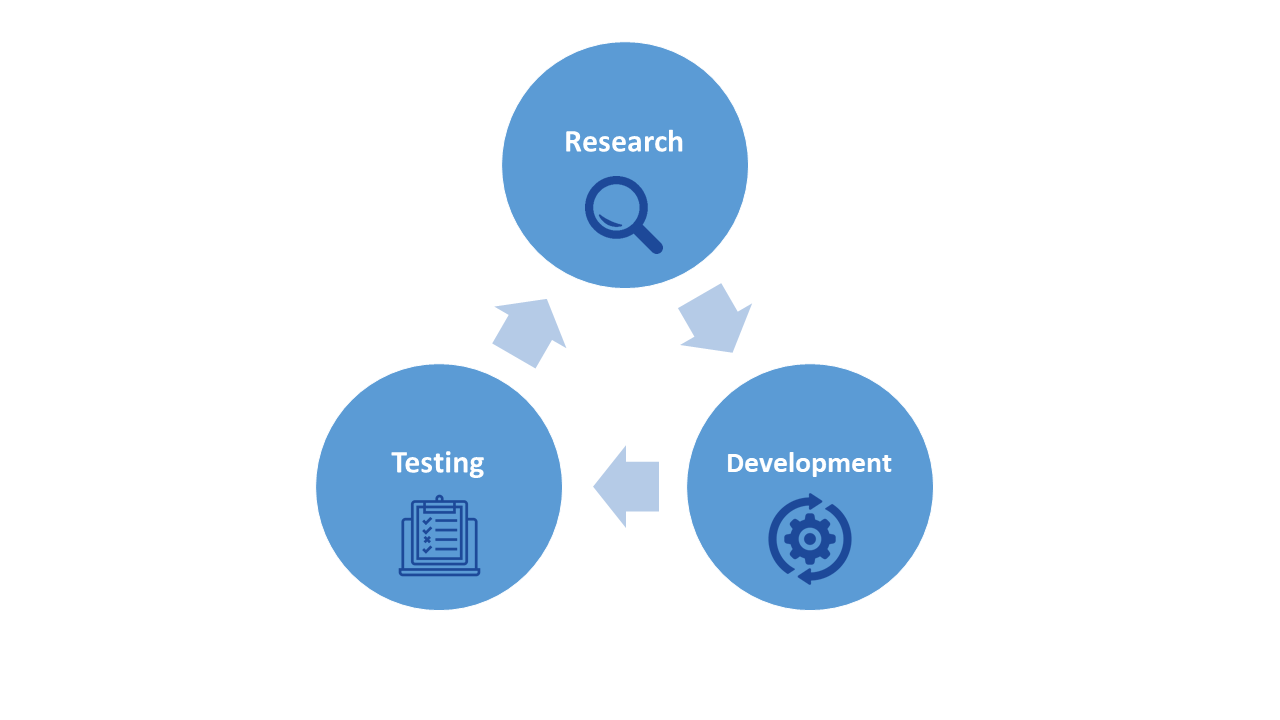
\includegraphics[height=2.5in,width=1\linewidth]{Chapters/Figures/r&d.png}}%
  \caption{Work Approach}
  \label{fig:WorkApp}
\end{figure}
% section document_structure (end)

% section Research Method (end)
\newpage
% section Research Questions
\section{Research Questions} % (fold)
\label{sec:research_question}

The purpose of this research is to evaluate if a wearable device, with a dynamic geolocation,  based in various system factors such as available communication, and power management, can contribute for an improved localization process and position accuracy. Where the main problem is to know the location of such devices, there is solutions based on GNSS and in this thesis will work as a reference, for a GNSS free alternative. The application of an adaptive geolocation solution for elderly people raises the following research problem:

\begin{itemize}
	\item \textbf{RQ:} What is the impact of~\gls{LPWAN} enabled solutions in wearable devices, especially those dedicated for people with dementia?
\end{itemize} 
% section research_questions (end)

% section Hypothesis
\section{Hypothesis}
\label{sec:hypothesis}

Can LPWAN enabled solutions, helping in perform the location of the person, while saving battery, reducing the overall cost, and complain with the technical constraints of a wearable devices. Having also the possibility to dynamically choose, the best location available in that moment.




% section Hypothesis (end)
%\section{Dissertation Plan}
%\label{sec:dissertation_plan}
%In this section the description of the work done is presented with a Gantt chart\ref{fig:gantt1} were the tasks and temporal planning for them is also presented.


%%%%%%%%%%% Gantt Chart figure Remove Possible %%%%%%%%%%
%begin{landscape}
%\begin{figure}[htbp]
%	\centering
%	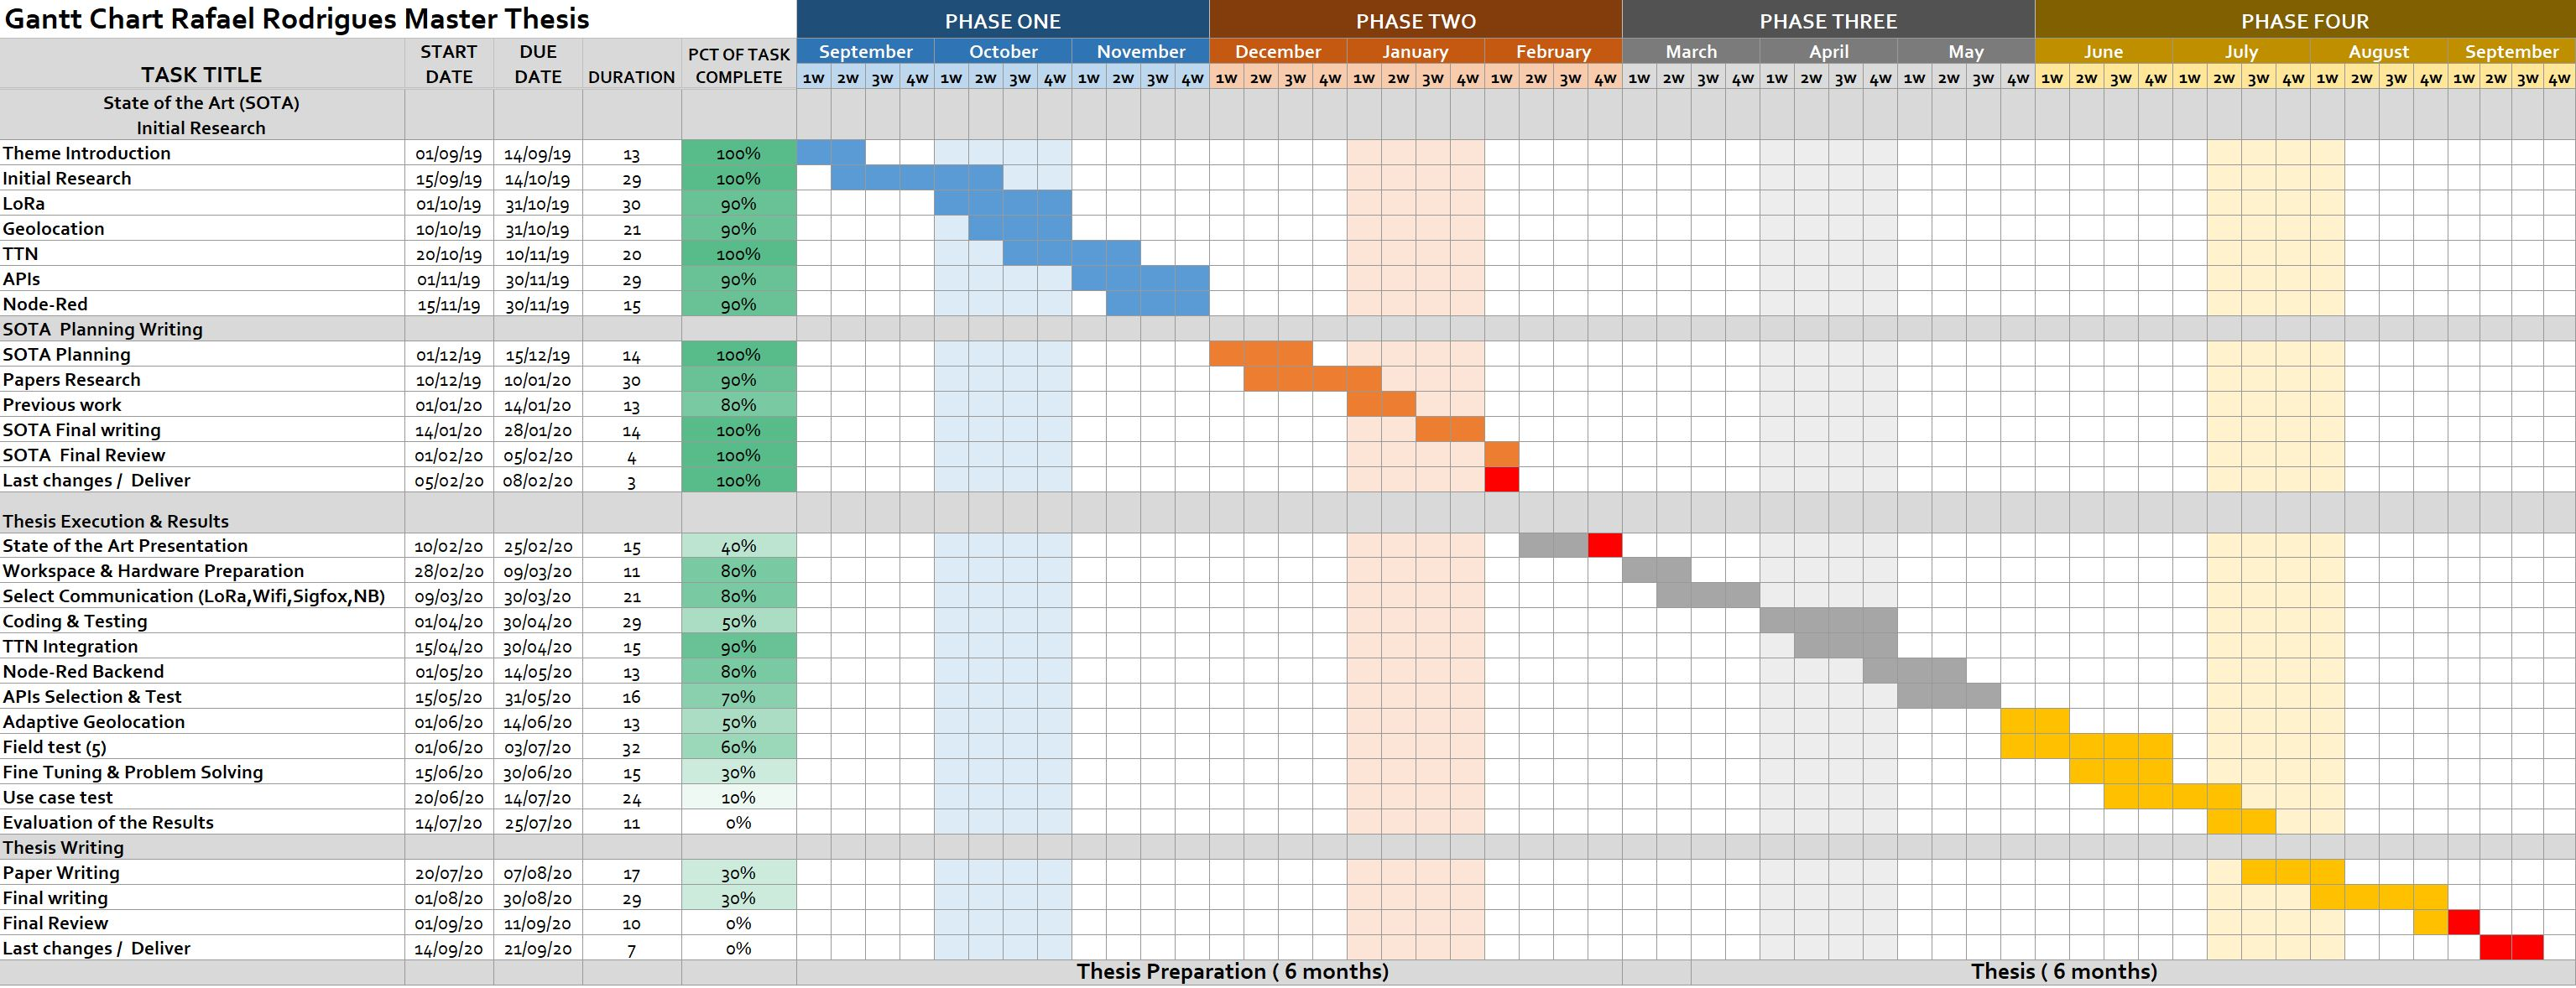
\includegraphics[height=6in,width=10.3in,angle=0]{Chapte%rs/Figures/GantJan2020.JPG}
%	\caption{Gantt Chart}
%	\label{fig:gantt1}
%\end{figure}
%\end{landscape}
%\newpage
%%%%%%%%%%%%%%%%%%%%%%%%%

% section Dissertation Outline
\section{Dissertation Outline}
\label{sec:dissertaion_outline}
This dissertation is dived in 6 chapters, which are presented bellow:


\begin{itemize}
	\item \textbf{Chapter 1 - Introduction}: This chapter describes the purpose of this dissertation as well as the motivation behind this research project. It also reveals the adopted research method. In addition,  presents the research question that motivated this work and its hypothesis, in order to solve this question;
	
	
	\item \textbf{Chapter 2 - State of the Art}: This chapter is used to describe the State of the Art for this dissertation. It represents the information that was necessary to have in order to build one model capable of validate the defined hypothesis.
	To do that, first, an overview is made of the current solutions for people with dementia. Next, it is described several LPWAN that can be used for the communication of geolocation data. After that, it is shown the different Geolocation Algorithms and methods. 
	Finally, it is described how LPWAN can be used for adaptive geolocation, and the similar work already done is introduced. 
	
	
	\item \textbf{Chapter 3 - Adaptive Geolocation}: This chapter, explain in detail the approach for the  proposed model,presenting the architecture of the system, where the model is working, and the modules to be implemented. 
	
	
	\item \textbf{Chapter 4 - Implementation}:  In  this chapter is described  the implementation of each part, with the technologies and methodology used.
	
	
	\item \textbf{Chapter 5 - Results}: This fifth chapter, presents the methodology used for the solution and the  proposed used case is presented, as well as the practical field tests, conducted for the project. 
	
	\item \textbf{Chapter 6 - Conclusions}: This dissertation is concluded with the presentation of the final thoughts and remarks, as well as the hypothesis presented for solving of the research question and problems previously identified. In the end of this chapter, a subsection "Future Work"~\ref{sec:Future_work} is presented with the propose for possible continuation work. 

\end{itemize}



% section Dissertation Outline (end)
%\newpage
% section Contributions
%\section{Contributions} % (fold)
%\label{sec:contribution}
%(Possivelmente esta parte é para eliminar)
%The author of this thesis presents the following contributions:\\
%escrever o que é original e o que é do projecto

%pacheco 2019
% section contributions (end)

%\subsection{Pycom} % (fold)
%\label{sec:pycom}
%The hardware used for this work will be later presented in a more detailed way, but these boards allows the use of a higher-level language, in this case, a shrink version of Python, because is running an interpreter that is MicroPython, so is possible now to program a  microcontroller in higher level, this as some benefits, for  example, the faster time from a prototype to the final product.

%image pycom 

% sub section  Pycom  (end)

%\subsection{Lora Gateway} % (fold)
%\label{sec:lora_Gateway}
%In order to realize the this thesis LoRa connectivity was required so the author deployed a LoRa gateway in the university, giving LoRa coverage to all campus, and in annex will be a guide in how this was done, helping now future work with this technology. 

% sub section  Pycom  (end)
%\subsection{Use Case} % (fold)
%\label{sec:use_case}
%This use case will also be explained in more detailed later in this document, but the purposed use case where this thesis is being developed is Carelink project in which the main focus will be to do a personal tracking device for people with dementia this project will be used for testing and validation of the results obtained during this thesis~\cite{carelink}

%\subsection{Relation To The Electrical And Computers Engineering} % (fold)
%\label{sec:relation}
